
% NC: Might need to have a think about how many tables and figures to include. Fine for thesis but please check JEB guidelines.
	%SF: Manuscript limit is 10 printed pages including figures and tables


%Start: 22/04/14
%Last edited on 01/08
	%Removed the simulations completely and changed the focus to more of a morphological study


% Preamble
% NC: I've reordered this a bit (but check it) so that stuff you'll always want is near the top
% and stuff you may need to change depending on the journal is near the bottom

\documentclass[12pt,a4paper]{article}
\usepackage{enumerate} 	% put in numbers or bullet points
\usepackage{setspace}	% line spacing					
\usepackage{authblk}	% For author affiliations
\usepackage{graphicx} 	% For adding pictures

\usepackage[nomarkers]{endfloat} %Figures and tables at the end of the document
\usepackage{pdflscape}	% for landscape pages
\usepackage{mathtools}	% For equations etc.
\usepackage[osf]{mathpazo} % palatino font package

\usepackage{ms}     	% load the manuscript style template

%\usepackage{float}		% Use these options to have figures in specific places in the text
%\floatstyle{plaintop} 	% Force table captions to go above the table

\setcounter{secnumdepth}{0} % removes numbers from section headings
\raggedright 			% justify the text on the left only
\pagenumbering{arabic}	% Page numbers

%\onehalfspacing 		%1.5 line spacing - use the below instead in case you need double spacing for some journals
%\linespread{1.6} 		% this is 1.5 spacing, double line spacing is 1.6 - unrecognised command (maybe due to the setspace package?)
\usepackage[round]{natbib} % author-year citations in round brackets

\title{Quantifying cranial morphological disparity in tenrecs (Afrosoricida, 	Tenrecidae) with implications for their designation as an adaptive radiation} 
% I want to come up with a better title

\author{Sive Finlay$^{1,2,*}$ and Natalie Cooper$^{1,2}$}
\affiliation{\noindent{\footnotesize
$^1$ School of Natural Sciences, Trinity College Dublin, Dublin 2, Ireland.\\ 
$^2$ Trinity Centre for Biodiversity Research, Trinity College Dublin, Dublin 2, Ireland.\\
$^*$sfinlay@tcd.ie; Zoology Building, Trinity College Dublin, Dublin 2, Ireland.\\ Fax: +353 1 6778094; Tel: +353 1 896 2571.\\}}
\date{}	% To give blank date

\runninghead{???} %I'll fix this when I have a proper title

\keywords{disparity, morphology, geometric morphometrics, tenrecs, golden moles, adaptive radiation}

% Start of document
\begin{document}

\modulolinenumbers[1] 	% Line numbering on every line

\mstitlepage			% Instead of \maketitle you can use the nice template to get it looking like a manuscript
\parindent=1.5em		% Changes paragraph indenting so it's not so big
\addtolength{\parskip}{.3em} % Changes spacing between sections so it's smaller
%---------------------------------------------------
\begin{abstract}
%I'll do this section last
\end{abstract}

\newpage
%-------------------------------------------------------
\section{Introduction} 

	Phenotypically diverse groups have long attracted the attentions of evolutionary biologists. Studies which quantify phenotypic variety \citep[e.g.][]{Price2013, Collar2011, Brusatte2008}  have important implications for understanding the factors that contribute to high morphological diversity in some groups and not others \citep{Losos2010a}. 

	These approaches are particularly relevant when it comes to the study of adaptive radiations: "evolutionary divergence of members of a single phylogenetic lineage into a variety of different adaptive forms" \citep[Futuyma 1998, cited by][]{Losos2010}. 
	There are many famous examples of adaptively radiated groups \citep{Gavrilets2009}. However, there has also been considerable debate about how adaptive radiations should be defined \citep{Glor2010, Losos2010a} based on the relative importance of speciation rate, species richness and morphological diversity. One particular issue is whether it is even meaningful to classify a specific group of species as an adaptive radiation or not since any classification relies on arbitrary distinctions between what are most likely a continua of characteristics which describe the diversity of a particular clade \citep{Olson2009}.

	However, despite the controversies and disagreements, there does seem to be a consensus that high morphological diversity is an important criterion for identifying a group of species as belonging on the adaptive radiation scale \citep{Losos2010a, Olson2009}. One way to test whether a group shows high morphological diversity is through sister taxa comparisons. For example, Losos and Miles (\citeyear{Losos2002}) used this approach to demonstrate exceptional diversity in some but not all clades of iguanid lizards.
%Probably needs another linking sentence here
	Here we use sister-taxa comparisons to test whether tenrecs (Afrosoricida, Tenrecidae) exhibit the high levels of phenotypic diversity that are expected of an adaptively radiated clade.

	The tenrec family is comprised of 34 species, 31 of which are endemic to Madagascar \citep{Olson2013}. From a single common ancestor \citep{Asher2006}, Malagasy tenrecs diversified into a wide variety of descendant species which convergently resemble distantly related insectivore mammals such as shrews (\textit{Microgale} tenrecs), moles (\textit{Oryzorictes} tenrecs) and hedgehogs (\textit{Echinops} and \textit{Setifer} tenrecs) \citep{Eisenberg1969}. These convergent resemblances are so great that tenrecs used to be considered part of the general "insectivore" clade and only molecular studies revealed their true phylogenetic affinites within the Afrotherian mammals \citep{Stanhope1998}.  

	Tenrecs are often cited as an example of an adaptively radiated family which exhibits exceptional morphological diversity \citep{Soarimalala2011, Olson2003, Eisenberg1969}. However, this apparent exceptional diversity has not been tested. Here we present the first quantitative test of patterns of phenotypic diversity in tenrecs and examine how morphological diversity in tenrecs compares to their closest relatives, the golden moles (Afrosoricida, Chryscholoridae). 

	We use disparity, the diversity of organic form \citep{Foote1997, Wills1994, Erwin2007}, to measure phenotypic variety within the two families. There is no single definition of disparity and it can be calculated in many ways including measures of morphospace occupation \citep[e.g.][]{Goswami2011, Brusatte2008} and rate-based approaches that assess the amount of directed change away from an ancestor \citep{OMeara2006, Price2013}. Here we focus on patterns of phenotypic variety in extant species rather than analysing the rate of diversity accumulation through time. 
	Using the most complete morphological data set of tenrecs and golden moles to date we apply two dimensional geometric morphometrics \citep{Rohlf1993, Adams2013} to quantify variation in cranial and mandible morphologies as proxies for phenotypic diversity in the two families. 

	Our results indicate an overall trend of higher morphological diversity in tenrec compared to golden mole crania. However, most of these differences are not statistically significant, indicating that, with regards to cranial shape, tenrecs are not as phenotypically diverse as is often assumed. In contrast, we found significantly greater morphological disparity in golden mole mandibles compared to tenrecs, seemingly due to more variable posterior mandible morphologies in golden moles.
	
	These findings cast doubt over whether the apparent phenotypic diversity within tenrecs should be considered to be truly exceptional. 


%-------------------------------------------------------------
\section{Materials and Methods}

\subsection{Morphological data collection} 

	%I've changed to including all 4 views in the main text of the paper because I had some more room after taking out the simulations. I think it makes more sense to have all of them together instead of separated in the paper and supplementary.
	
	One of us (SF) photographed cranial specimens of tenrecs and golden moles at the Natural History Museum London (NHML), the Smithsonian Institute Natural History Museum (SI), the American Museum of Natural History (AMNH), Harvard's Museum of Comparative Zoology (MCZ) and the Field Museum of Natural History, Chicago (FMNH). We photographed the specimens with a Canon EOS 650D camera fitted with an EF 100mm f/2.8 Macro USM lens using a standardised procedure to minimise potential error (see supplementary material for details). 
	%NC Might want to use the standard museum abbreviations - BMNH etc.
		%SF I used NHML because I thought the BMNH was the old name?

	We collected pictures of the skulls in dorsal, ventral and lateral views (right side of the skull) and of the outer (buccal) side of the right mandibles. A full list of museum accession numbers and details for how to access the images can be found in the supplementary material.
	%AMNH and SI pictures are on figshare but MCZ and FMNH are more tricky about copyright so I haven't put those pictures up

	In total we collected pictures from 182 skulls in dorsal view (148 tenrecs and 34 golden moles), 173 skulls in ventral view (141 tenrecs and 32 golden moles), 171 skulls in lateral view (140 tenrecs and 31 golden moles)   and 182 mandibles in lateral view (147 tenrecs and 35 golden moles), representing 31 species of tenrec (out of the total 34 in the family) and 12 species of golden moles (out of a total of 21 in the family \citep{Asher2010}). %I could put all of this into a table?
	We used the taxonomy of Wilson and Reeder \citeyearpar{Wilson2005} supplemented with more recent sources \citep{IUCN2012, Olson2013} to identify our specimens. 
	

	We used a combination of both landmarks (type 2 and type 3, \citep{Zelditch2012}) and semilandmarks to characterise the shapes of our specimens. Figure \ref{fig:skdors_skvent_landmarks} shows our landmarks (points) and semilandmarks (outline curves) for the skulls in dorsal and ventral views and figure \ref{fig:sklat_mands_landmarks} shows the points and curves we used for lateral views of skulls and mandibles. Corresponding definitions of each of the landmarks can be found in the supplementary material.
	
	%I thought the four tables of definitions would take up too much space here?
	

	We digitised all landmarks and semilandmarks in tpsDIG, version 2.17 \citep{Rohlf2013}. We re-sampled the outlines to the minimum number of evenly spaced semilandmark points required to represent each outline accurately \citep[][details in supplementary material]{MacLeod2013}. We used TPSUtil \citep{Rohlf2012} to create sliders files \citep{Zelditch2012} to define which points were semilandmarks. We conducted all subsequent analyses in R version 3.0.2 \citep{Team2014} within the geomorph package \citep{Adams2013}. We used the gpagen function to run a general Procrustes alignment \citep{Rohlf1993} of the landmark coordinates while sliding the semilandmarks by minimising procrustes distance \citep{Bookstein1997}. We used these Procrustes-aligned coordinates of all species to calculate average shape values for each species (n=43) which we then used for a principal components (PC) analysis with the plotTangentSpace function \citep{Adams2013}. 

%*************************************************
%May need to re-do pictures to grey scale instead of colour

%**************************************
%Skdors and skvent
	%landmarks diagram
	\begin{figure}
	\centering
	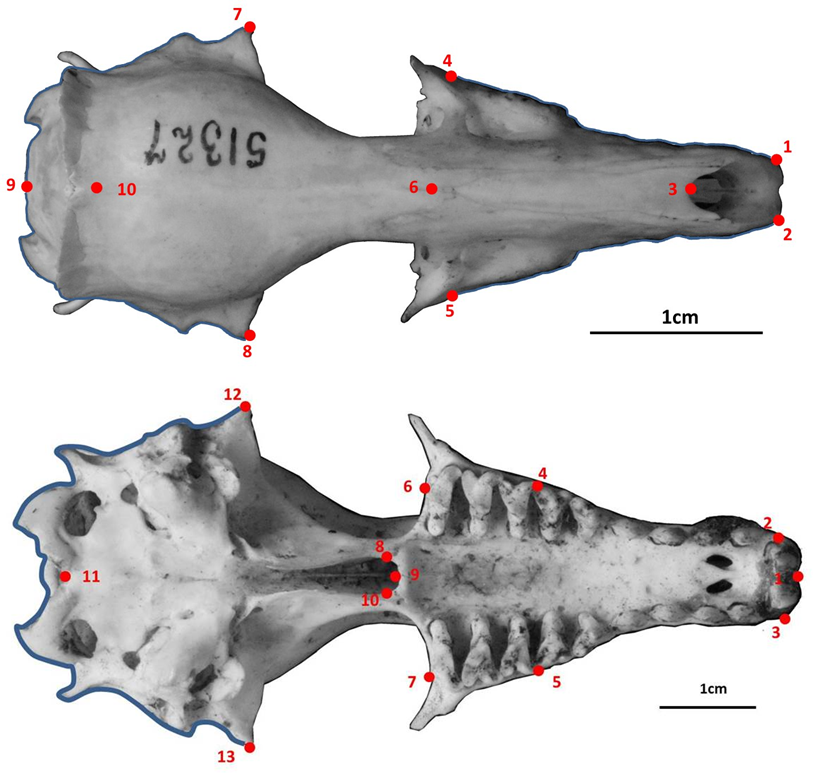
\includegraphics[width=1\linewidth]{figures/SkDors+Skvent_landmark_diagrams.png}
	
	\caption[Diagram of the landmarks and curves for the skulls in dorsal and ventral views]
		{Landmarks (red points) and curves (blue lines) used to capture the morphological shape of skulls in dorsal and ventral views respectively. Curves were re-sampled to the same number of evenly-spaced points. Descriptions of the curves and landmarks are in the supplementary material. The specimens belong to two different \textit{Potamogale velox} (Tenrecidae) skulls: accession number AMNH 51327 for the dorsal picture and NHML 1934.6.16.2 for the ventral picture}
	
	\label{fig:skdors_skvent_landmarks}
	\end{figure}


%Mandibles and Skulls lateral
	%landmarks diagram
	\begin{figure}[H]
	\centering
	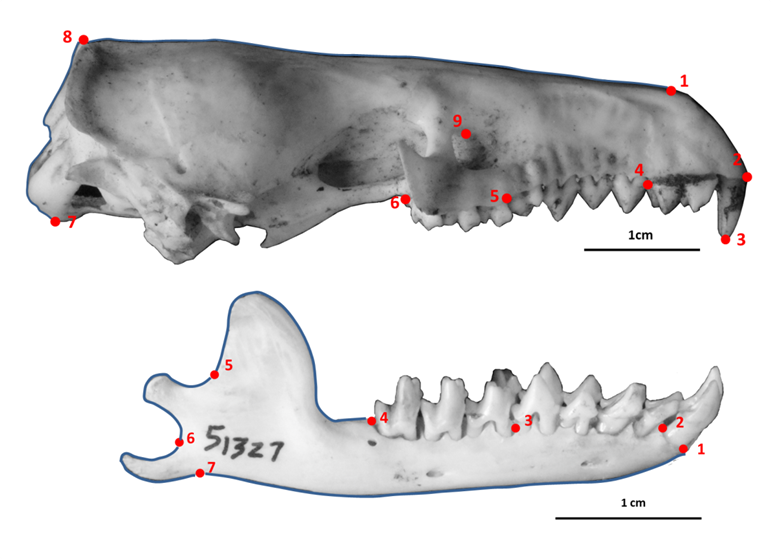
\includegraphics[width=1\linewidth]{figures/SkLat+mands_landmark_diagrams.png}
	
	\caption[Diagrams of the landmarks and curves used for lateral views of skulls and mandibles]
		{Landmarks (red points) and curves (blue lines) used to capture the morphological shape of lateral views of skulls and mandibles respectively. Curves were re-sampled to the same number of evenly-spaced points. Descriptions of the curves and landmarks are in the supplementary material.The specimens belong to two different \textit{Potamogale velox} (Tenrecidae) skulls: accession number AMNH 51327 for the dorsal picture and NHML 1934.6.16.2 for the ventral picture}
	
	\label{fig:sklat_mands_landmarks}
	\end{figure}
%

%************************************************** 
%I'm no longer using the phylogenies for comparing disparity in the two families - they were just for the simulations part

%I don't know if it's necessary to do phylogenetic PCAs since I'm already basing all of my comparisons on family divisions?

%\subsubsection{Phylogeny} 
	%Instead of basing our analyses on individual trees and assuming that their topologies were known without error \citep[e.g.][]{Ruta2013, Foth2012, Brusatte2008, Harmon2003} we used a distribution of 101 pruned phylogenies derived from the randomly resolved mammalian supertrees in \citep{Kuhn2011}. 
		% I used 101 because that was the number in the smaller Fritz file - I could change it to 100 instead if 101 sounds odd?

	%Eight species (six \textit{Microgale} tenrecs and two golden moles) in our morphological data were not in the phylogenies. Phylogenetic relationships among the \textit{Microgale} have not been resolved more recently than the \citep{Kuhn2011} analysis, therefore we added the additional \textit{Microgale} species at random to the \textit{Microgale} genus within each phylogeny \citep{Revell2012}. We could not use the same approach to add the two missing golden mole species because they were the only representatives of their respective genera within our data. Therefore we randomly added these species to the common ancestral node (using the findMRCA function in phytools \citep{Revell2012}) of all golden moles within each phylogeny. Adding these extra species to the phylogenies created polytomies which we resolved arbitrarily using zero-length branches \citep{Paradis2004}. We calculated pairwise phylogenetic distances among species using the cophenetic function \citep{Team2014}. 
	% NC: I feel like some of this belongs in the analysis section...
		%SF Me too but I'm not sure where to put it without making a separate analyses section for the phylogenies and I don't think that makes sense.  
	
%-------------------------------------------------------	
\subsection{Disparity calculations}

	We calculated morphological disparity separately for golden moles and tenrecs in each of the morphological datasets. We used the PC axes which accounted for 95\% of the cumulative variation to calculate four disparity metrics; the sum and product of the range and variance of morphospace occupied by each family \citep{Brusatte2008, Foth2012, Ruta2013}. We also calculated morphological disparity directly from the Procrustes-superimposed shape data based on the sum of the squared inter-landmark distances between the average shape of a species and the overall grand mean shape \citep[SSqDist,][]{Zelditch2012}. 

	We used two approaches to test whether tenrecs have significantly different morphologies compared to golden moles. The first was a comparison of morphospace occupation between the two groups with non parametric MANOVAs \citep{Anderson2001} to test whether tenrecs and golden moles occupy significantly different areas of morphospace \citep[e.g][]{Serb2011, Ruta2013}.
	 
	Secondly, we used pairwise permutation tests to test the null hypothesis that tenrecs and golden moles have equal disparity. If this hypothesis were true then the designation of each species as belonging to either tenrecs or golden moles should be arbitrary. Therefore we permutated the data by assigning family identities at random to each specimen and calculated the differences in disparity for each of the new family groupings. We repeated these permutations 1000 times to generate a null distribution of the expected differences in family disparity. We compared our observed (true) measures of the differences in disparity between tenrecs and golden moles to these permutated distributions to test whether the families had significantly different levels of disparity.

	The majority of tenrec species (19 out of 31 in our data) are members of the \textit{Microgale} (shrew-like) genus which is notable for its relatively low phenotypic diversity \citep{ Soarimalala2011, Jenkins2003}. The strong similarities among these species may mask signals of higher disparity among other tenrecs. Therefore we repeated our family-level comparisons of disparity with a reduced data set that excluded the \textit{Microgale} so that we could compare disparity within the remaining 12 tenrec species to disparity within the 12 species of golden moles.


%-----------------------------------------------------------

\section{Results}


\subsection{Morphological disparity in tenrecs and golden moles} 
 
	Figure  \ref{fig:fourPCA} depicts the morphospace plots derived from our principal components analyses of average Procrustes-superimposed shape coordinates for each species in our skull and mandible data respectively. We used the principal components axes which accounted for 95\% of the cumulative variation (n = 7, 8, 8 axes for the dorsal, ventral and lateral skull analyses respectively and n = 12 axes for the mandibles) to calculate the disparity of each family. 

	Tenrecs and golden moles clearly have very different cranial and mandible morphologies: in each analysis, the families occupy significantly different areas of morphospace (npMANOVA, table \ref{tab:npmanova.summary}). 
	Our comparisons of disparity levels within each family yielded different trends for the skulls compared to the mandible analyses.
	
	In our analyses of the three different views of the skulls, when disparity is calculated from principal component - based metrics there is an overall trend for tenrecs to have higher disparity than golden moles. However, none of these differences are statistically significant (table \ref{tab:disp.summary}). 
	
	In contrast, when we calculated disparity based on the squared inter-landmark distances between the average shape of a species and the overall grand mean shape \citep{Zelditch2012} then golden moles had significantly higher levels of disparity than tenrecs (table \ref{tab:disp.summary}). These results indicate that golden moles are more distant from the overall mean shape in each of the analyses (farther from the (0,0) points in the PCA plots figure \ref{fig:fourPCA}) which makes intuitive sense given that the overall meanshape in each analysis will necessarily be biased towards the more species-rich tenrec family. 
	
	%I'm not sure if this is the right interpretation of the SSqDist results because I thought the permutation tests take sample size differences into account? 
	%I could just take out this extra metric completely to avoid confusion
	
	There is a less clear pattern from our analysis of disparity in the mandibles. Three of our five metrics indicate that golden moles have significantly higher disparity in the shape of their mandibles than tenrecs (table \ref{tab:disp.summary}) although one metric (sum of ranges) indicated the opposite result. 
	
	The three curves at the back of the mandibles (figure \ref{fig:sklat_mands_landmarks}) place a particular emphasis on shape variation in the posterior of the bone; the ramus, coronoid, condylar and angular processes. Therefore, higher disparity in golden mole mandibles compared to tenrecs could be driven by greater morphological variation in these structures. To test this idea, we repeated our morphometric analyses of the mandibles with a reduced data set of points; just the seven landmark points and one single curve at the base of the jaw between landmarks 1 and 7 (figure \ref{fig:sklat_mands_landmarks}). When we compared familial disparity levels with this reduced data set we found that golden moles no longer had significantly higher disparity than tenrecs but rather there were some indications that the opposite was true (table \ref{tab:disp.summary}).
	
\subsection{Morphological disparity in non-\textit{Microgale} tenrecs and golden moles} 	   
	
	We repeated our disparity comparisons with a subset of the tenrec specimens to remove the large and phenotypically similar \textit{Microgale} tenrec genus. In this case we found that tenrecs have significantly higher disparity than golden moles when the skulls are analysed in lateral view (table \ref{tab:disp.nonmic.summary}). However, none of the other comparisons in any of the analyses were significant. Similarly, the trend in the main analysis for golden moles to have significantly higher disparity measured as the sum of squared inter-landmark distances (table \ref{tab:disp.summary}) was not repeated in this comparison of disparity in non-\textit{Microgale} tenrecs and golden moles (table \ref{tab:disp.nonmic.summary}).


%************************************
%Results tables and figures

%Summary table of the family comparisons for all tenrecs vs. golden moles
	\begin{table}[h]			
	\caption[Summary of disparity comparisons between tenrecs and golden moles]
		{Summary of disparity comparisons between tenrecs (T) and golden moles (G) for each of our data sets(rows) and five disparity metrics (columns). "Mandibles:one curve" refers to our shape analysis of mandibles excluding the three curves around the posterior structures of jaw (figure \ref{fig:sklat_mands_landmarks}). Significant differences are highlighted in bold with the corresponding p value in brackets. Disparity metrics are; sum of variance, product of variance, sum of ranges, product of ranges and sum of squared distances among species. }
	\centering
	%Disparity family comparison results summary
%All tenrecs and golden moles

\begin{tabular}[t]{l l l l l l }		
\hline
\textbf{Disparity metric} & \textbf{SumVar} & \textbf{ProdVar} & \textbf{SumRange} & \textbf{ProdRange} & \textbf{SSqDist} \\
\hline
Skulls dorsal & T$>$G & T$>$G & T$>$G & T$>$G &	\textbf{G$>$T* (0)}\\
%-----------------------------------------------------------
Skulls lateral	& T$>$G & T$>$G & T$>$G & T$>$G & \textbf{G$>$T* (0)}\\
%-------------------------------------------------------
Skulls ventral & T$>$G & G$>$T & T$>$G & T$>$G & \textbf{G$>$T* (0)}\\
%-------------------------------------------------------
Mandibles & G$>$T & \textbf{G$>$T* (0.008)} & \textbf{T$>$G* (0.025)} & \textbf{T$>$G* (0.009)} &	\textbf{T$>$G* (0)}\\
%-------------------------------------------------------
Mandibles: one curve & G$>$T & G$>$T & T$>$G & T$>$G &	\textbf{T$>$G* (0)}\\
%-------------------------------------------------------
\hline
\end{tabular} 
	\label{tab:disp.summary}  
	\end{table}

%Summary of the family comparisons for non-Microgale tenrecs vs. golden moles
	\begin{table}[h]			
	\caption[Summary of disparity comparisons between non-\textit{Microgale} tenrecs and golden moles]
		{Summary of disparity comparisons between non-\textit{Microgale} tenrecs (T) and golden moles (G) for each of our data sets(rows) and five disparity metrics (columns). Significant differences are highlighted in bold with the corresponding p value in brackets. Disparity metrics are; sum of variance, product of variance, sum of ranges, product of ranges and sum of squared distances among species. }
	\centering
	%Disparity family comparison results summary
%Non-Microgale tenrecs and golden moles

\begin{tabular}[t]{l l l l l l }		
\hline
\textbf{Disparity metric} & \textbf{SumVar} & \textbf{ProdVar} & \textbf{SumRange} & \textbf{ProdRange} & \textbf{SSqDist} \\
\hline
Skulls dorsal & T$>$G & T$>$G & T$>$G & T$>$G &	T$>$G\\
%-----------------------------------------------------------
Skulls lateral	& T$>$G* (0.014) & T$>$G & \textbf{T$>$G* (0.001)} & \textbf{T$>$G*(0.003)} & \textbf{G$>$T* (0.014)}\\
%-------------------------------------------------------
Skulls ventral & T$>$G & T$>$G & T$>$G & T$>$G & T$>$G\\
%-------------------------------------------------------
Mandibles & T$>$G & G$>$T & T$>$G & G$>$T &	G$>$T\\
%-------------------------------------------------------
%Don't need to do a subset analysis of mandibles for non-Microgale tenrecs
%Mandibles one curve & G$>$T & T$>$G & T$>$G & T$>$G & G$>$T\\
%-------------------------------------------------------
\hline
\end{tabular} 
	\label{tab:disp.nonmic.summary}  
	\end{table}
	
%Summary table of the npMANOVA morphospace occupation comparisons
	
	\begin{table}[h]			

	\caption[Summary of npMANOVA comparisons of morphospace occupation for tenrecs and golden moles]
		{Summary of the npMANOVA comparisons of morphospace occupation for tenrecs and golden moles in each of the four analyses (three views of skulls and mandibles). In each case the two families occupy significantly different areas of morphospace.}
	\centering
	
%All tenrecs and golden moles
%npMANOVA results summary
%Values from the _manova.res files: npMANOVA based on the PC axes (not distance matrices)

\begin{tabular}[t]{l l l l }		
\hline
\textbf{Analysis} & \textbf{F} & R$^2$ & p value \\
\hline
Skulls dorsal & 66.02 & 0.62 & 0.001 \\
%-------------------------------------------
Skulls ventral & 100.74 & 0.71 &0.001 \\
%------------------------------------------
Skulls lateral & 75.07 & 0.65 & 0.001 \\
%------------------------------------
Mandibles & 59.34 & 0.59 & 0.001 \\
%-------------------------------------------------------
\hline
\end{tabular} 
	\label{tab:npmanova.summary}  
	\end{table}
		
%PCA figures: changed to having all four plots instead of individual PCA graphs
	%Source of this figure in my shape_data/output folder 
	\begin{figure}[H]
	\centering
	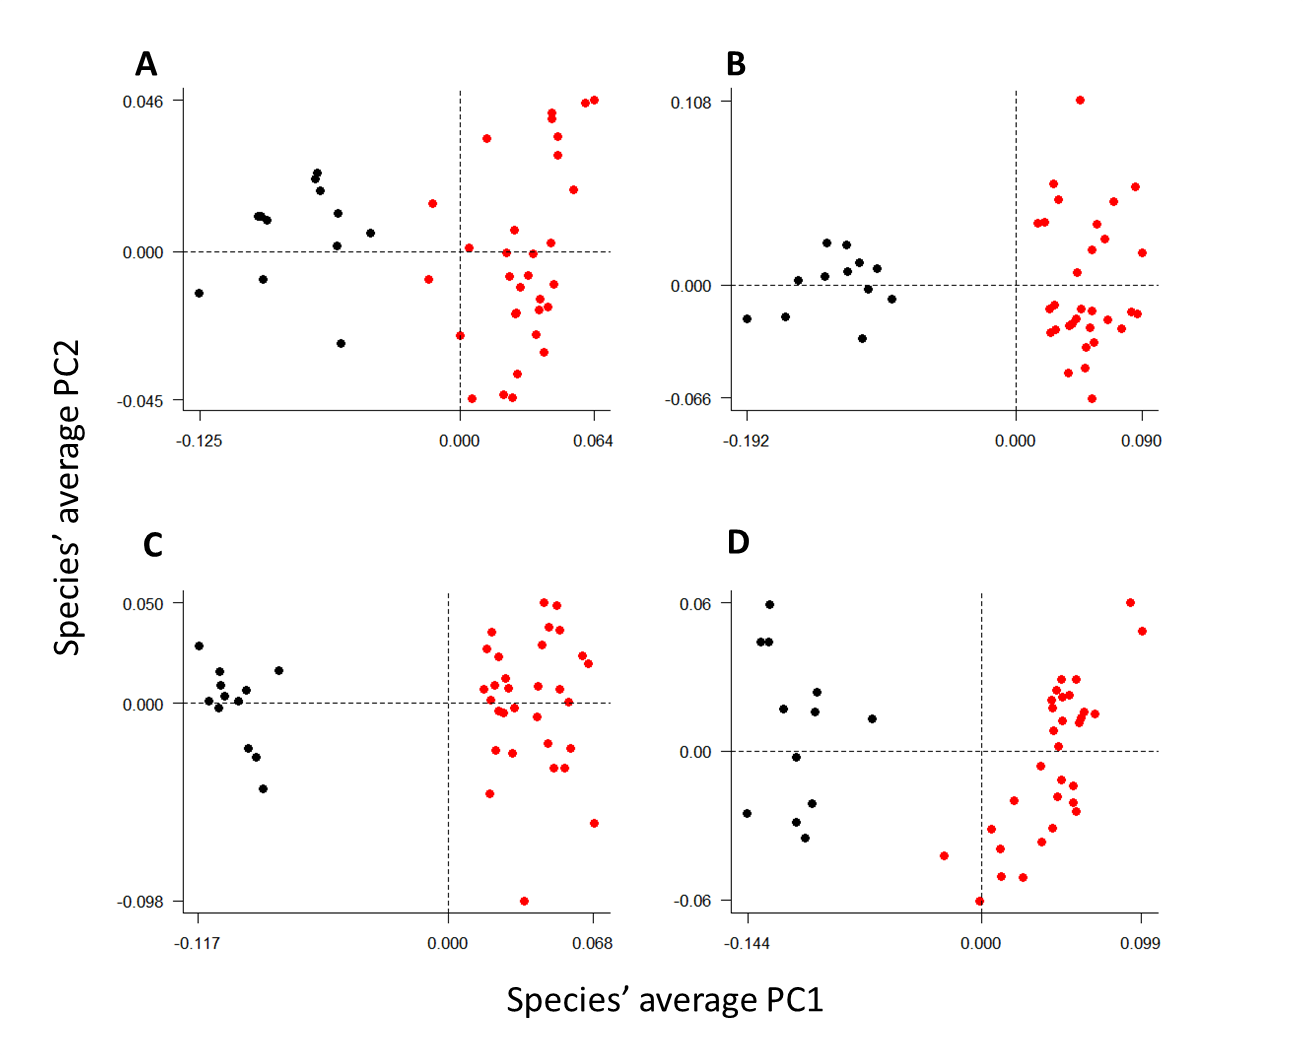
\includegraphics[width=1\linewidth]{figures/FourPlotPCA.png}
	\caption[Principal components plots of the morphospaces occupied by tenrecs and golden moles]
		{Principal components plots of the morphospaces occupied by tenrecs (red, n=31 species) and golden moles (black, n=12) for the skulls: dorsal (A), ventral (B), lateral (C) and mandibles (D) analyses. Axes are PC1 and PC2 of the average scores from a PCA analysis of mean Procrustes shape coordinates for each species. }
	\label{fig:fourPCA}
	\end{figure}
%**********************************************


\section{Discussion} 


	Here we presented the first quantitative investigatio of morphlogical disparity in terencs and our results suggest that phenotypic variation in tenrecs is not as exceptional as it first appears.
	 
	When we compared tenrecs' cranial morphologies to their closest relatives we found a trend towards higher disparity in tenrecs than in golden moles but none of these differences were significant. In contrast, the analyses of the mandibles indicated that golden moles have more disparate mandible shapes than tenrecs seemingly due to greater diversity within their posterior-mandible shapes.

	
	It is evident that tenrecs are a diverse group, both phenotypically and ecologically. Body sizes of extant tenrecs span three orders of magnitude (2.5 to $>$ 2,000g) which is a greater range than all other Families, and most Orders, of living mammals \citep{Olson2003}. Within this vast size range there is striking phenotypic diversity, from the spiny \textit{Echinops, Setifer} and striking \textit{Hemicentetes} to the shrew-like  \textit{Microgale}. Furthermore, tenrecs inhabit a variety of ecological niches and habitats including terrestrial, arboreal, semi-aquatic and semi-fossorial forms \citep{Soarimalala2011}. 
	In contrast, although golden moles occupy a wide altitudinal, climatic and vegetational spectrum of habitats \citep{Bronner1995}, they are are all fossorial species which, superficially at least, appear to be less phenotypically diverse than tenrecs. 
	
	There is a danger when using sister taxa comparisons that a clade's diversity will be judged to be exceptional just because it is more variable than an exceptionally non-diverse sister taxa \citep{Losos2002}. However, we compared an apparently phenotypically diverse clade to a more uniform sister taxa yet our results do not indicate that tenrecs are more morphologically diverse than their closest relatives (table \ref{tab:disp.summary}). 
	
	%Needs another sentence here
	
   

	%2: Why are there opposite patterns in the skulls and mandibles?
	
	%I asked for advice from Gary Bronner about why I was getting higher variation in golden mole mandibles compared to tenrecs. He thinks that the most likely reason is a problem with my landmarks. Landmark 4 is the alveolus of the last molar but that position is not homologous across species because of the presence/absence of a third molar. His advice was to re-run the analysis without landmark 4 and curve A and see what patterns of shape variation come out then.
	
	%However, as I was choosing the landmarks I knew that the dental formulae varied for each species - and therefore the landmarks are relative points showing the end of the tooth row rather than biologically meaningful positions of dental characteristics. But now I don't know if I can get away with using that as an excuse when it comes to trying to explain strange results in my paper.
	
	One apparent anomaly in our results is that we found opposite patterns of group dissimilarities in the analyses of skulls and mandibles. 
	Our landmarks and curves for the mandibles (figure \ref{fig:sklat_mands_landmarks}) include aspects of variation in the dentition but they focus particular attention on the ascending ramus (condyloid, condylar and angular processes). Therefore higher disparity in golden moles could reflect greater morphological variability in these posterior mandible structures. To test this idea we deleted the three semi-landmark curves around these structures and repated our disparity analyses of mandibles using seven landmarks and just one curve at the base of the jaw. In this case we retrieved the opposite pattern than previously: tenrecs had higher morphological disparity than golden moles (see supplementary material). Therefore, our results indicate that golden moles have greater morphological variation in the posterior structures of their mandibles compared to tenrecs.
	
		%NB; I still need to add these results to the supplementary
	%Needs another sentence here
		
 	It proved impossible to position reliable landmarks on the corresponding mandibular articulation areas of the skull in lateral view (see supplementary). Therefore we could not test whether higher morphological disparity in the rami were correlated with associated morphological variety in the articulation areas of the skull.
	
	
	%The discrepancies could arise from factors associated with the modularity of morphological evolution.

	%There is strong evidence that morphological variation in skulls and mandibles is derived from differential evolution of integrated developmental modules \citep[reviewed by][]{Klingenberg2013a}.
	%For example, there seems to be two primary modules in the mouse mandible; an alveolar part which holds the teeth and the ascending ramus for muscle attachment and which articulates with the skull \citep{Klingenberg2008a}. Geometric shape covariation is stronger within rather than between these modules. 



%4 - Caveats

 	Evidence of exceptional morphological diversity is one criterion for designating a clade as an adaptive radiation \citep{Losos2010a} and our analyses are the first measures of morphological diversity within tenrecs, a group which is commonly cited as an example of an adaptive radiation \citep{Olson2013}.  However, describing phenotypic divergence as the product of an adaptive radiation requires exceptional morphological diversity in traits which have specific and proven adaptive significance \citep{Losos2010a}. We have not included any measures of the "adaptiveness" of cranial shape in our analyses and therefore our analyses should not be considered to be an explicit test of whether tenrecs are an adaptive radiation or not. 
 	
 	The evolution of cranial shape (both upper skull and mandible), particularly dental morphology, has obvious correlations with dietary specialisations (REFS) and occupation of specific ecological niches (REFS). Considering the wide ecological diversity of our study species; semi-fossorial, arboreal, terrestrial and semi-aquatic tenrecs \citep{Soarimalala2011} we think that it is reasonable to expect that this variety should be reflected in skull morphology. Future work should focus on explicit measures of the "adaptiveness" and functional importance of tenrec cranial and post-cranial morphologies to understand the significance of morphological diversity within the family \citep[e.g.][]{Mahler2010}. 

	Studies of morphological disparity are inevitably constrained to measure diversity within specific traits rather than overall phenotypes \citep{Roy1997}. Here we focused on cranial morphology, tratis which are commonly used to delineate species boundaries (REFS) or for cross-taxonomic comparative studies of phenotypic (dis)similarities (REFS). Disparity caculations based on skull shape can yield similar results compared to analyses of whole-skeleton discrete characters and limb proportion data sets \citep{Foth2012}. 
	
	However, we would need to extend our analyses to other morphological proxies of phenotype to test whether the cranial morphological disparity patterns presented here are indicative of overall differences in phenotypic diversity in tenrecs and golden moles. 
	



%5 - Implications

	These results highlight the importance of applying quantitative methods to testing our assumptions about adaptively radiated groups. 

	%Put in the Gavrilets and Losos 2009 point that it's important to expand our studies of adaptive radiation to different cases and not just the typical examples
	%Ruta 2013: ecological opportunity doesn't necessariliy correlate with increased morphological disparity

	These analyses represent the first attempt to find evidence to support the common claim that tenrecs are an adaptive radiation. Future work will develop our results by expanding the analyses to non-cranial morphology and also measures of ecological diversity. However, our current results provide a clear indication that phenotypic variety within tenrecs is perhaps not as exceptional as it first seems and therefore their designation as an adaptive radiation may need to be re-considered.



%Of course cranial diversity is only one aspect of morphological dispariy and more analyses are needed but this is still interesting/relevant because it's the first to test whether phenotypic diversity in tenrecs is more than skin deep/greater than expected by chance

\section*{Acknowledgements}

	We thank Fran\c{c}ois Gould, Dean Adams, David Polly, Gary Bronner, Steve Brusatte, Steve Wang, Luke Harmon, Thomas Guillerme and the members of NERD club for insightful discussions and the musuem staff and curators for their support and access to collections. Funding was provided by an Irish Research Council EMBARK Initiative Postgraduate Scholarship (SF) and the European Commission CORDIS Seventh Framework Programme (FP7) Marie Curie CIG grant. Proposal number: 321696 (NC, SF)

\bibliographystyle{jeb}
\bibliography{refs_disparity}
% I downloaded the jeb.bst file from http://schneider.ncifcrf.gov/latex.html but there isn't an associated style file

% NC: You can make one via the command line as I showed you in one of my LaTeX lessons.

	%**********************
	%SF: I still need to do this so that the references have the abbreviated journal titles, don't include the doi and don't include the total number of pages in books
	%*******************************************




\end{document}